\documentclass{standalone}
\usepackage{tikz}
\usetikzlibrary{patterns, positioning}


\begin{document}
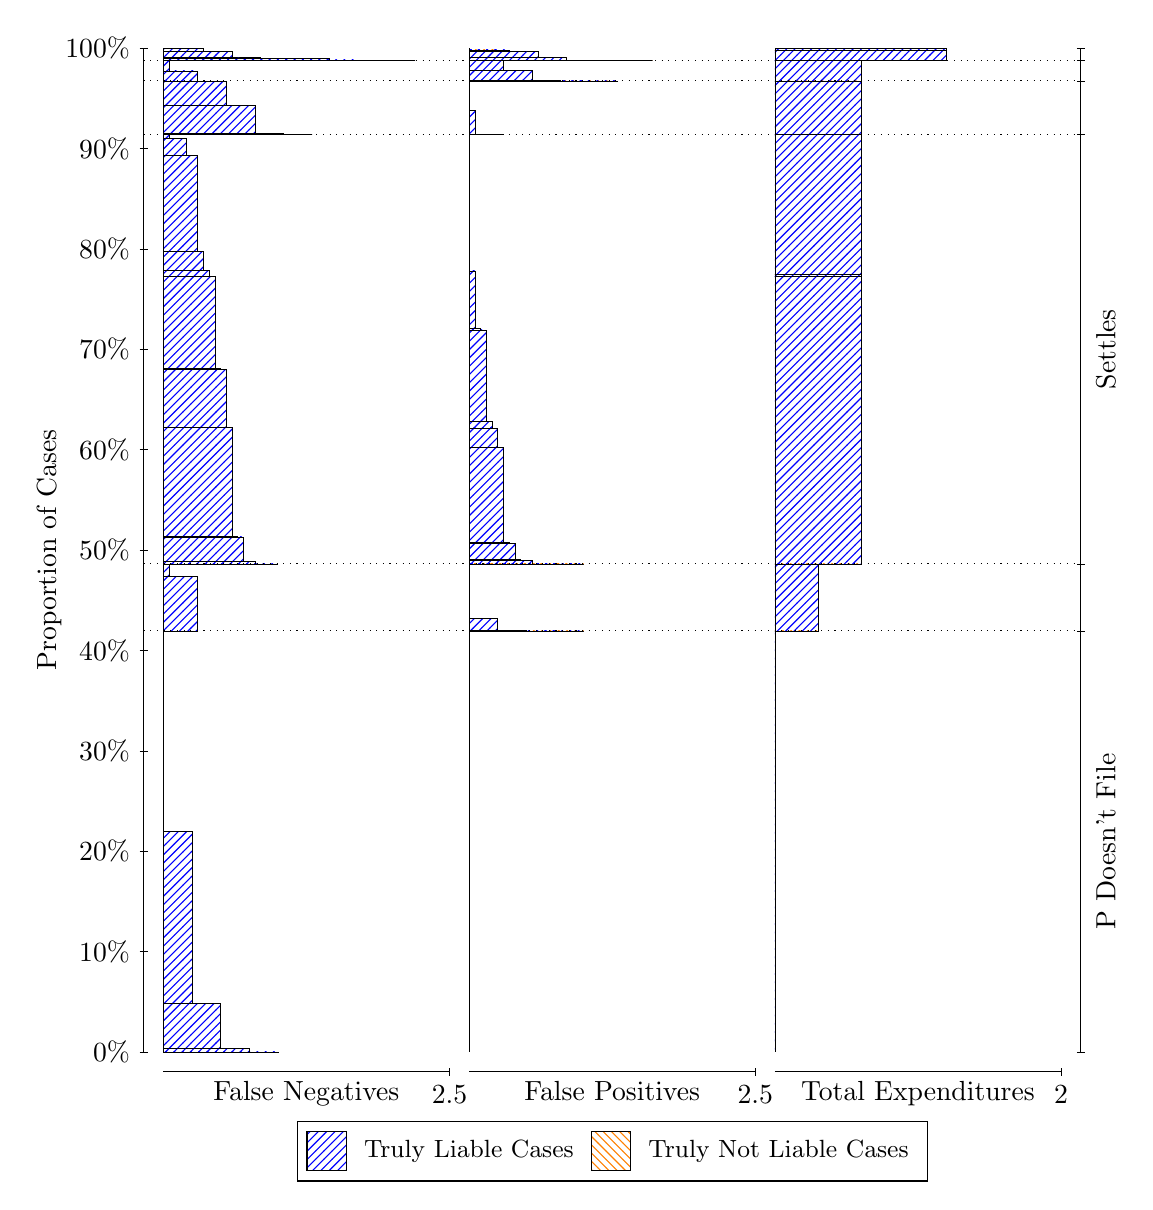
\begin{tikzpicture}
\draw[black, very thin] (1.5,1.75) -- (1.5,14.5);
\node[rotate=90, text=black, anchor=center] at (0.3, 8.125) {Proportion of Cases};
\draw[black, very thin] (1.45,1.75) -- (1.55,1.75);
\node[text=black, anchor=east] at (1.45, 1.75) {0\%};
\draw[black, very thin] (1.45,3.025) -- (1.55,3.025);
\node[text=black, anchor=east] at (1.45, 3.025) {10\%};
\draw[black, very thin] (1.45,4.3) -- (1.55,4.3);
\node[text=black, anchor=east] at (1.45, 4.3) {20\%};
\draw[black, very thin] (1.45,5.575) -- (1.55,5.575);
\node[text=black, anchor=east] at (1.45, 5.575) {30\%};
\draw[black, very thin] (1.45,6.85) -- (1.55,6.85);
\node[text=black, anchor=east] at (1.45, 6.85) {40\%};
\draw[black, very thin] (1.45,8.125) -- (1.55,8.125);
\node[text=black, anchor=east] at (1.45, 8.125) {50\%};
\draw[black, very thin] (1.45,9.4) -- (1.55,9.4);
\node[text=black, anchor=east] at (1.45, 9.4) {60\%};
\draw[black, very thin] (1.45,10.675) -- (1.55,10.675);
\node[text=black, anchor=east] at (1.45, 10.675) {70\%};
\draw[black, very thin] (1.45,11.95) -- (1.55,11.95);
\node[text=black, anchor=east] at (1.45, 11.95) {80\%};
\draw[black, very thin] (1.45,13.225) -- (1.55,13.225);
\node[text=black, anchor=east] at (1.45, 13.225) {90\%};
\draw[black, very thin] (1.45,14.5) -- (1.55,14.5);
\node[text=black, anchor=east] at (1.45, 14.5) {100\%};

\draw[black, very thin] (13.4,1.75) -- (13.4,14.5);
\draw[black, very thin] (13.35,1.75) -- (13.45,1.75);
\node[anchor=west] at (13.35, 1.75) {};
\draw[black, very thin] (13.35,7.0988) -- (13.45,7.0988);
\node[anchor=west] at (13.35, 7.0988) {};
\draw[black, very thin] (13.35,7.9482) -- (13.45,7.9482);
\node[anchor=west] at (13.35, 7.9482) {};
\draw[black, very thin] (13.35,13.404) -- (13.45,13.404);
\node[anchor=west] at (13.35, 13.404) {};
\draw[black, very thin] (13.35,14.083) -- (13.45,14.083);
\node[anchor=west] at (13.35, 14.083) {};
\draw[black, very thin] (13.35,14.344) -- (13.45,14.344);
\node[anchor=west] at (13.35, 14.344) {};
\draw[black, very thin] (13.35,14.5) -- (13.45,14.5);
\node[anchor=west] at (13.35, 14.5) {};

\draw[black, very thin, pattern color=blue, pattern=north east lines] (1.75,1.75) rectangle (3.2033,1.7504);
\draw[black, very thin, pattern color=blue, pattern=north east lines] (1.75,1.7504) rectangle (2.84,1.7932);
\draw[black, very thin, pattern color=blue, pattern=north east lines] (1.75,1.7932) rectangle (2.4767,2.3682);
\draw[black, very thin, pattern color=blue, pattern=north east lines] (1.75,2.3682) rectangle (2.1133,4.5524);
\draw[black, very thin, pattern color=orange, pattern=north west lines] (1.75,4.5524) rectangle (1.75,4.5524);
\draw[black, very thin, pattern color=blue, pattern=north east lines] (1.75,4.5524) rectangle (1.75,7.0988);
\draw[black, very thin, pattern color=blue, pattern=north east lines] (1.75,7.0988) rectangle (2.186,7.7945);
\draw[black, very thin, pattern color=blue, pattern=north east lines] (1.75,7.7945) rectangle (1.8227,7.944);
\draw[black, very thin, pattern color=orange, pattern=north west lines] (1.75,7.944) rectangle (1.75,7.944);
\draw[black, very thin, pattern color=blue, pattern=north east lines] (1.75,7.944) rectangle (1.75,7.9482);
\draw[black, very thin, pattern color=blue, pattern=north east lines] (1.75,7.9482) rectangle (3.2033,7.9482);
\draw[black, very thin, pattern color=blue, pattern=north east lines] (1.75,7.9482) rectangle (3.058,7.9482);
\draw[black, very thin, pattern color=blue, pattern=north east lines] (1.75,7.9482) rectangle (2.9127,7.9772);
\draw[black, very thin, pattern color=blue, pattern=north east lines] (1.75,7.9772) rectangle (2.84,7.9777);
\draw[black, very thin, pattern color=blue, pattern=north east lines] (1.75,7.9777) rectangle (2.7673,8.2912);
\draw[black, very thin, pattern color=blue, pattern=north east lines] (1.75,8.2912) rectangle (2.6947,8.3001);
\draw[black, very thin, pattern color=blue, pattern=north east lines] (1.75,8.3001) rectangle (2.622,9.6835);
\draw[black, very thin, pattern color=blue, pattern=north east lines] (1.75,9.6835) rectangle (2.5493,10.418);
\draw[black, very thin, pattern color=blue, pattern=north east lines] (1.75,10.418) rectangle (2.4767,10.432);
\draw[black, very thin, pattern color=blue, pattern=north east lines] (1.75,10.432) rectangle (2.404,11.599);
\draw[black, very thin, pattern color=blue, pattern=north east lines] (1.75,11.599) rectangle (2.3313,11.675);
\draw[black, very thin, pattern color=blue, pattern=north east lines] (1.75,11.675) rectangle (2.2587,11.92);
\draw[black, very thin, pattern color=blue, pattern=north east lines] (1.75,11.92) rectangle (2.186,13.133);
\draw[black, very thin, pattern color=blue, pattern=north east lines] (1.75,13.133) rectangle (2.1133,13.139);
\draw[black, very thin, pattern color=blue, pattern=north east lines] (1.75,13.139) rectangle (2.0407,13.351);
\draw[black, very thin, pattern color=blue, pattern=north east lines] (1.75,13.351) rectangle (1.968,13.355);
\draw[black, very thin, pattern color=blue, pattern=north east lines] (1.75,13.355) rectangle (1.8953,13.356);
\draw[black, very thin, pattern color=blue, pattern=north east lines] (1.75,13.356) rectangle (1.8227,13.404);
\draw[black, very thin, pattern color=orange, pattern=north west lines] (1.75,13.404) rectangle (1.75,13.404);
\draw[black, very thin, pattern color=blue, pattern=north east lines] (1.75,13.404) rectangle (1.75,13.404);
\draw[black, very thin, pattern color=blue, pattern=north east lines] (1.75,13.404) rectangle (3.6393,13.404);
\draw[black, very thin, pattern color=blue, pattern=north east lines] (1.75,13.404) rectangle (3.276,13.413);
\draw[black, very thin, pattern color=blue, pattern=north east lines] (1.75,13.413) rectangle (2.9127,13.774);
\draw[black, very thin, pattern color=blue, pattern=north east lines] (1.75,13.774) rectangle (2.5493,14.079);
\draw[black, very thin, pattern color=blue, pattern=north east lines] (1.75,14.079) rectangle (2.186,14.083);
\draw[black, very thin, pattern color=orange, pattern=north west lines] (1.75,14.083) rectangle (1.75,14.083);
\draw[black, very thin, pattern color=blue, pattern=north east lines] (1.75,14.083) rectangle (2.186,14.209);
\draw[black, very thin, pattern color=blue, pattern=north east lines] (1.75,14.209) rectangle (1.8227,14.34);
\draw[black, very thin, pattern color=orange, pattern=north west lines] (1.75,14.34) rectangle (1.75,14.34);
\draw[black, very thin, pattern color=blue, pattern=north east lines] (1.75,14.34) rectangle (1.75,14.344);
\draw[black, very thin, pattern color=blue, pattern=north east lines] (1.75,14.344) rectangle (4.9473,14.344);
\draw[black, very thin, pattern color=blue, pattern=north east lines] (1.75,14.344) rectangle (4.584,14.344);
\draw[black, very thin, pattern color=blue, pattern=north east lines] (1.75,14.344) rectangle (4.2207,14.348);
\draw[black, very thin, pattern color=blue, pattern=north east lines] (1.75,14.348) rectangle (3.8573,14.365);
\draw[black, very thin, pattern color=blue, pattern=north east lines] (1.75,14.365) rectangle (3.712,14.365);
\draw[black, very thin, pattern color=blue, pattern=north east lines] (1.75,14.365) rectangle (3.494,14.367);
\draw[black, very thin, pattern color=blue, pattern=north east lines] (1.75,14.367) rectangle (3.3487,14.367);
\draw[black, very thin, pattern color=blue, pattern=north east lines] (1.75,14.367) rectangle (3.1307,14.367);
\draw[black, very thin, pattern color=blue, pattern=north east lines] (1.75,14.367) rectangle (2.9853,14.386);
\draw[black, very thin, pattern color=blue, pattern=north east lines] (1.75,14.386) rectangle (2.7673,14.386);
\draw[black, very thin, pattern color=blue, pattern=north east lines] (1.75,14.386) rectangle (2.622,14.462);
\draw[black, very thin, pattern color=blue, pattern=north east lines] (1.75,14.462) rectangle (2.2587,14.498);
\draw[black, very thin, pattern color=blue, pattern=north east lines] (1.75,14.498) rectangle (1.8953,14.5);
\draw[black, very thin, pattern color=orange, pattern=north west lines] (1.75,14.5) rectangle (1.75,14.5);
\draw[black, very thin, pattern color=blue, pattern=north east lines] (1.75,14.5) rectangle (1.75,14.5);
\draw[black, very thin, pattern color=orange, pattern=north west lines] (5.6333,1.75) rectangle (5.6333,1.75);
\draw[black, very thin, pattern color=blue, pattern=north east lines] (5.6333,1.75) rectangle (5.6333,7.0988);
\draw[black, very thin, pattern color=orange, pattern=north west lines] (5.6333,7.0988) rectangle (7.0867,7.0988);
\draw[black, very thin, pattern color=blue, pattern=north east lines] (5.6333,7.0988) rectangle (7.0867,7.0988);
\draw[black, very thin, pattern color=blue, pattern=north east lines] (5.6333,7.0988) rectangle (6.7233,7.0988);
\draw[black, very thin, pattern color=blue, pattern=north east lines] (5.6333,7.0988) rectangle (6.36,7.1029);
\draw[black, very thin, pattern color=blue, pattern=north east lines] (5.6333,7.1029) rectangle (5.9967,7.2525);
\draw[black, very thin, pattern color=blue, pattern=north east lines] (5.6333,7.2525) rectangle (5.6333,7.9482);
\draw[black, very thin, pattern color=orange, pattern=north west lines] (5.6333,7.9482) rectangle (7.0867,7.9482);
\draw[black, very thin, pattern color=blue, pattern=north east lines] (5.6333,7.9482) rectangle (7.0867,7.9482);
\draw[black, very thin, pattern color=orange, pattern=north west lines] (5.6333,7.9482) rectangle (6.9413,7.9482);
\draw[black, very thin, pattern color=blue, pattern=north east lines] (5.6333,7.9482) rectangle (6.9413,7.9482);
\draw[black, very thin, pattern color=orange, pattern=north west lines] (5.6333,7.9482) rectangle (6.796,7.9482);
\draw[black, very thin, pattern color=blue, pattern=north east lines] (5.6333,7.9482) rectangle (6.796,7.9482);
\draw[black, very thin, pattern color=blue, pattern=north east lines] (5.6333,7.9482) rectangle (6.7233,7.9482);
\draw[black, very thin, pattern color=orange, pattern=north west lines] (5.6333,7.9482) rectangle (6.6507,7.9482);
\draw[black, very thin, pattern color=blue, pattern=north east lines] (5.6333,7.9482) rectangle (6.6507,7.9482);
\draw[black, very thin, pattern color=blue, pattern=north east lines] (5.6333,7.9482) rectangle (6.578,7.9485);
\draw[black, very thin, pattern color=orange, pattern=north west lines] (5.6333,7.9485) rectangle (6.5053,7.9485);
\draw[black, very thin, pattern color=blue, pattern=north east lines] (5.6333,7.9485) rectangle (6.5053,7.9485);
\draw[black, very thin, pattern color=blue, pattern=north east lines] (5.6333,7.9485) rectangle (6.4327,7.9962);
\draw[black, very thin, pattern color=blue, pattern=north east lines] (5.6333,7.9962) rectangle (6.36,7.9974);
\draw[black, very thin, pattern color=blue, pattern=north east lines] (5.6333,7.9974) rectangle (6.2873,8.0012);
\draw[black, very thin, pattern color=blue, pattern=north east lines] (5.6333,8.0012) rectangle (6.2147,8.2136);
\draw[black, very thin, pattern color=blue, pattern=north east lines] (5.6333,8.2136) rectangle (6.142,8.2195);
\draw[black, very thin, pattern color=blue, pattern=north east lines] (5.6333,8.2195) rectangle (6.0693,9.4326);
\draw[black, very thin, pattern color=blue, pattern=north east lines] (5.6333,9.4326) rectangle (5.9967,9.6772);
\draw[black, very thin, pattern color=blue, pattern=north east lines] (5.6333,9.6772) rectangle (5.924,9.7535);
\draw[black, very thin, pattern color=blue, pattern=north east lines] (5.6333,9.7535) rectangle (5.8513,10.921);
\draw[black, very thin, pattern color=blue, pattern=north east lines] (5.6333,10.921) rectangle (5.7787,10.935);
\draw[black, very thin, pattern color=blue, pattern=north east lines] (5.6333,10.935) rectangle (5.706,11.669);
\draw[black, very thin, pattern color=blue, pattern=north east lines] (5.6333,11.669) rectangle (5.6333,13.404);
\draw[black, very thin, pattern color=orange, pattern=north west lines] (5.6333,13.404) rectangle (6.0693,13.404);
\draw[black, very thin, pattern color=blue, pattern=north east lines] (5.6333,13.404) rectangle (6.0693,13.408);
\draw[black, very thin, pattern color=blue, pattern=north east lines] (5.6333,13.408) rectangle (5.706,13.713);
\draw[black, very thin, pattern color=blue, pattern=north east lines] (5.6333,13.713) rectangle (5.6333,14.083);
\draw[black, very thin, pattern color=orange, pattern=north west lines] (5.6333,14.083) rectangle (7.5227,14.083);
\draw[black, very thin, pattern color=blue, pattern=north east lines] (5.6333,14.083) rectangle (7.5227,14.083);
\draw[black, very thin, pattern color=blue, pattern=north east lines] (5.6333,14.083) rectangle (7.1593,14.083);
\draw[black, very thin, pattern color=blue, pattern=north east lines] (5.6333,14.083) rectangle (6.796,14.087);
\draw[black, very thin, pattern color=blue, pattern=north east lines] (5.6333,14.087) rectangle (6.4327,14.218);
\draw[black, very thin, pattern color=blue, pattern=north east lines] (5.6333,14.218) rectangle (6.0693,14.344);
\draw[black, very thin, pattern color=orange, pattern=north west lines] (5.6333,14.344) rectangle (7.9587,14.344);
\draw[black, very thin, pattern color=blue, pattern=north east lines] (5.6333,14.344) rectangle (7.9587,14.344);
\draw[black, very thin, pattern color=orange, pattern=north west lines] (5.6333,14.344) rectangle (7.5953,14.344);
\draw[black, very thin, pattern color=blue, pattern=north east lines] (5.6333,14.344) rectangle (7.5953,14.344);
\draw[black, very thin, pattern color=orange, pattern=north west lines] (5.6333,14.344) rectangle (7.232,14.344);
\draw[black, very thin, pattern color=blue, pattern=north east lines] (5.6333,14.344) rectangle (7.232,14.346);
\draw[black, very thin, pattern color=blue, pattern=north east lines] (5.6333,14.346) rectangle (6.8687,14.382);
\draw[black, very thin, pattern color=orange, pattern=north west lines] (5.6333,14.382) rectangle (6.8687,14.382);
\draw[black, very thin, pattern color=blue, pattern=north east lines] (5.6333,14.382) rectangle (6.8687,14.382);
\draw[black, very thin, pattern color=blue, pattern=north east lines] (5.6333,14.382) rectangle (6.5053,14.457);
\draw[black, very thin, pattern color=blue, pattern=north east lines] (5.6333,14.457) rectangle (6.5053,14.458);
\draw[black, very thin, pattern color=orange, pattern=north west lines] (5.6333,14.458) rectangle (6.36,14.458);
\draw[black, very thin, pattern color=blue, pattern=north east lines] (5.6333,14.458) rectangle (6.36,14.458);
\draw[black, very thin, pattern color=blue, pattern=north east lines] (5.6333,14.458) rectangle (6.142,14.468);
\draw[black, very thin, pattern color=blue, pattern=north east lines] (5.6333,14.468) rectangle (6.142,14.477);
\draw[black, very thin, pattern color=orange, pattern=north west lines] (5.6333,14.477) rectangle (5.9967,14.477);
\draw[black, very thin, pattern color=blue, pattern=north east lines] (5.6333,14.477) rectangle (5.9967,14.477);
\draw[black, very thin, pattern color=blue, pattern=north east lines] (5.6333,14.477) rectangle (5.7787,14.477);
\draw[black, very thin, pattern color=blue, pattern=north east lines] (5.6333,14.477) rectangle (5.7787,14.477);
\draw[black, very thin, pattern color=orange, pattern=north west lines] (5.6333,14.477) rectangle (5.6333,14.477);
\draw[black, very thin, pattern color=blue, pattern=north east lines] (5.6333,14.477) rectangle (5.6333,14.5);
\draw[black, very thin, pattern color=orange, pattern=north west lines] (9.5167,1.75) rectangle (9.5167,1.75);
\draw[black, very thin, pattern color=blue, pattern=north east lines] (9.5167,1.75) rectangle (9.5167,7.0988);
\draw[black, very thin, pattern color=orange, pattern=north west lines] (9.5167,7.0988) rectangle (10.062,7.0988);
\draw[black, very thin, pattern color=blue, pattern=north east lines] (9.5167,7.0988) rectangle (10.062,7.9482);
\draw[black, very thin, pattern color=orange, pattern=north west lines] (9.5167,7.9482) rectangle (10.607,7.9482);
\draw[black, very thin, pattern color=blue, pattern=north east lines] (9.5167,7.9482) rectangle (10.607,11.601);
\draw[black, very thin, pattern color=orange, pattern=north west lines] (9.5167,11.601) rectangle (10.607,11.601);
\draw[black, very thin, pattern color=blue, pattern=north east lines] (9.5167,11.601) rectangle (10.607,11.622);
\draw[black, very thin, pattern color=orange, pattern=north west lines] (9.5167,11.622) rectangle (10.607,11.622);
\draw[black, very thin, pattern color=blue, pattern=north east lines] (9.5167,11.622) rectangle (10.607,13.404);
\draw[black, very thin, pattern color=orange, pattern=north west lines] (9.5167,13.404) rectangle (10.607,13.404);
\draw[black, very thin, pattern color=blue, pattern=north east lines] (9.5167,13.404) rectangle (10.607,14.083);
\draw[black, very thin, pattern color=orange, pattern=north west lines] (9.5167,14.083) rectangle (10.607,14.083);
\draw[black, very thin, pattern color=blue, pattern=north east lines] (9.5167,14.083) rectangle (10.607,14.344);
\draw[black, very thin, pattern color=orange, pattern=north west lines] (9.5167,14.344) rectangle (11.697,14.344);
\draw[black, very thin, pattern color=blue, pattern=north east lines] (9.5167,14.344) rectangle (11.697,14.467);
\draw[black, very thin, pattern color=orange, pattern=north west lines] (9.5167,14.467) rectangle (11.697,14.467);
\draw[black, very thin, pattern color=blue, pattern=north east lines] (9.5167,14.467) rectangle (11.697,14.5);
\draw[black, dotted] (1.5,7.0988) -- (13.4,7.0988);
\draw[black, dotted] (1.5,7.9482) -- (13.4,7.9482);
\draw[black, dotted] (1.5,13.404) -- (13.4,13.404);
\draw[black, dotted] (1.5,14.083) -- (13.4,14.083);
\draw[black, dotted] (1.5,14.344) -- (13.4,14.344);
\draw[black, very thin] (1.75,1.5) -- (5.3833,1.5);
\node[text=black, anchor=north] at (3.5667, 1.5) {False Negatives};
\draw[black, very thin] (5.3833,1.45) -- (5.3833,1.55);
\node[text=black, anchor=north] at (5.3833, 1.45) {2.5};

\draw[black, very thin] (5.6333,1.5) -- (9.2667,1.5);
\node[text=black, anchor=north] at (7.45, 1.5) {False Positives};
\draw[black, very thin] (9.2667,1.45) -- (9.2667,1.55);
\node[text=black, anchor=north] at (9.2667, 1.45) {2.5};

\draw[black, very thin] (9.5167,1.5) -- (13.15,1.5);
\node[text=black, anchor=north] at (11.333, 1.5) {Total Expenditures};
\draw[black, very thin] (13.15,1.45) -- (13.15,1.55);
\node[text=black, anchor=north] at (13.15, 1.45) {2};

\node[text=black, centered, rotate=90] at (13.72, 4.4244) {P Doesn't File};

\node[text=black, centered, rotate=90] at (13.72, 10.676) {Settles};




\draw (7.449999999999999,1.5) node[draw=none] (baseCoordinate) {};
\begin{scope}[align=center]
        \matrix[scale=0.5, draw=black, below=0.5cm of baseCoordinate, nodes={draw}, column sep=0.1cm]{
            \node[rectangle, draw, minimum width=0.5cm, minimum height=0.5cm, pattern color=blue, pattern=north east lines] {}; &
            \node[draw=none, font=\small, text=black] (B) {Truly Liable Cases}; &
            \node[rectangle, draw, minimum width=0.5cm, minimum height=0.5cm, pattern color=orange, pattern=north west lines] {}; &
            \node[draw=none, font=\small, text=black] (B) {Truly Not Liable Cases}; \\
            };
\end{scope}

\end{tikzpicture}
\end{document}